\documentclass[a4paper,11pt]{article}
\usepackage[T1]{fontenc}
\usepackage[utf8]{inputenc}
\usepackage{lmodern}
\usepackage[francais]{babel}
\usepackage{geometry}
\usepackage{float}
\usepackage{array}
\usepackage{multirow}
\usepackage{makecell}
\usepackage{graphicx}
\usepackage{listings}
\usepackage{appendix}
\usepackage{amsmath}
\usepackage{comment}


\newcolumntype{M}[1]{>{\raggedright}m{#1}}

\geometry{hmargin=2.0cm,vmargin=1.5cm}

\title{Logique floue\\\texttt{Sauvons le RMS Titanic}}

\author{Alexis \textsc{Decker-Wurtz}, Erwan  \textsc{Duroux}, Guillaume  \textsc{Laroyenne}}

\begin{document}

    \maketitle

    \begin{abstract}
        Ce document présente une synthèse du projet de logique floue que nous avons réalisé en deuxième année.
        Le cœur de ce projet est une bibliothèque de logique floue que nous avons programmé en \textit{C++}. La bibliothèque comporte les principaux opérateurs de bases de la logique floue ainsi que quelques méthodes de défuzzification.
        Pour les utilisateurs puissent manipuler plus simplement cette bibliothèque, nous avons décidé d'ajouter un interpréteur permettant de modéliser des problèmes de logique floue sans avoir à la manipuler directement.
        La logique floue permettant de prendre des décisions complexe à partir d'un ensemble de données. Nous avons décidé de l'utiliser afin de réaliser un pilote automatique évitant les obstacles pouvant se trouver devant un navire, tout en utilisant la bibliothèque que nous avons conçu.
    \end{abstract}

    \section{Construction de la bibliothèque de logique floue}

    \begin{center}
        Pour toute information sur l'arborescence, la compilation et l'utilisation de la bibliothèque, veuillez vous référer au fichier \textbf{README.md} consultable à la racine du projet à l’adresse : \texttt{https://github.com/LaroyenneG/fuzzy-logic}
    \end{center}

    Notre \textit{framework} a été développé en langage \textit{C++} et compilé avec le compilateur GNU \textit{g++} et \textit{CMake}.
    Affin de s’assurer du bon fonctionnement de la bibliothèque, nous avons utilisé le \textit{framework} \textit{CPPUNIT} permettant de réaliser des tests unitaires en langage \textit{C++}.
    Toutes les opérandes et opérateurs sont vérifiés via un filet de test permettant d’identifier d’éventuel mauvais fonctionnement.
    Cela permet d'effectuer des modifications sur la librairie en identifiant rapidement les possibles régressions.

    \begin{figure}[H]
        \begin{center}
            \caption{UML des packages du \textit{framework} de logique floue}
            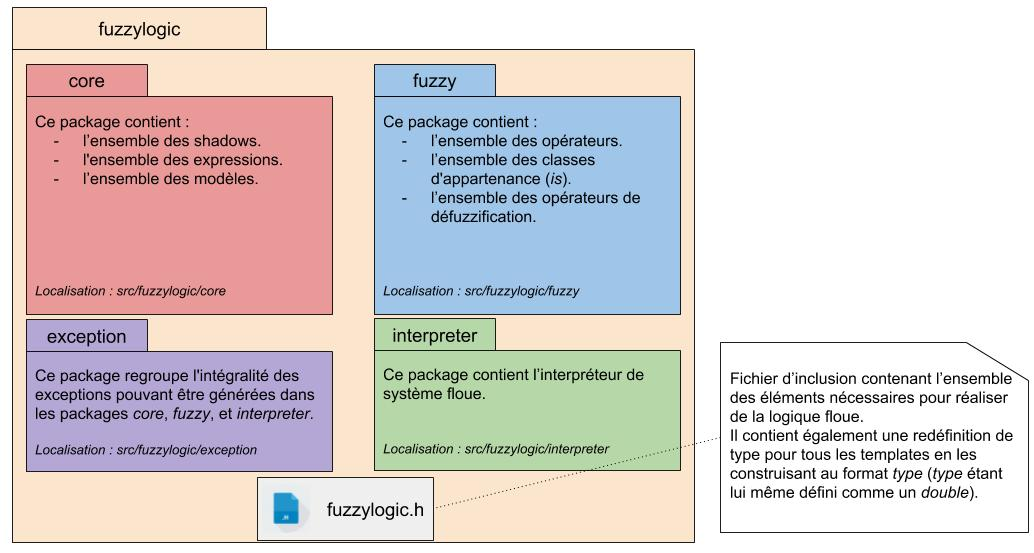
\includegraphics[scale=0.51]{assets/Packages_(UML).jpg}
            \label{fig:umlPackage}
        \end{center}
    \end{figure}


    \begin{table}[H]
        \caption{Liste des opérateurs est opérandes du \textit{framework} de logique floue}
        \label{tab:listing}

        \begin{center}
            \begin{tabular}{|c|c|M{4cm}|}
                \hline
                Nom & Type & Description \tabularnewline
                \hline
                AggPlus & Agg & Retourne l'addition des évaluations des valeurs d'entrées entre 0 et 1\tabularnewline
                \hline
                AggMax & Agg & Retourne la valeur maximale des évaluations des valeurs d'entrées\tabularnewline
                \hline
                AndMin & And & Retourne la valeur minimale des évaluations des valeurs d'entrées\tabularnewline
                \hline
                AndMult & And & Retourne la multiplication des évaluations des valeurs d'entrées\tabularnewline
                \hline
                ApproximatelyEqual & Or & Retourne la valeur de l'évaluation si les évaluations des valeurs d'entrées sont égales à 0,2 près sinon retourne zero\tabularnewline
                \hline
                Equal & Or & Retourne la valeur de l'évaluation si les évaluations des valeurs d'entrées sont égales sinon renvoi zero\tabularnewline
                \hline
                NotMinus1 & Not & Retourne la valeur de l'évaluation la résultat de 1 moins l'évaluation de l'opérateur\tabularnewline
                \hline
                OrMax & Or & Retourne la valeur maximale des évaluations des valeurs d'entrées\tabularnewline
                \hline
                OrPlus & Or & Retourne l'addition des évaluations des valeurs d'entrées entre 0 et 1\tabularnewline
                \hline
                ThenMin & Then & Retourne la valeur minimale des évaluations des valeurs d'entrées\tabularnewline
                \hline
                ThenMult & Then & Retourne la multiplication des évaluations des valeurs d'entrées\tabularnewline
                \hline
            \end{tabular}
        \end{center}
    \end{table}

    \section{Mise en place d'un interpréteur de logique floue}

    Pour réaliser des systémes floue plus simplement, nous avons réalisé un interpreteur utilisant notre bibliothéque.
    Il réalise les manipulations sur la factory en fonction des instructions d'un texte d'entrée,
    Cela permet de se rapprocher plus du langage humain, afin de se concentrer uniquement sur la logique et non de l'acepet programmation.

    \begin{figure}[H]
        \begin{center}
            \caption{Schéma présentant le concept de l'interpreteur}
            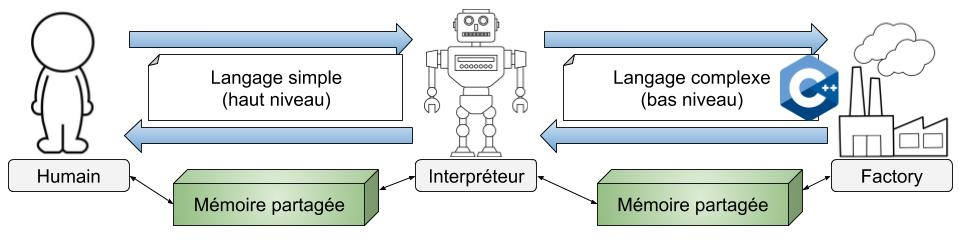
\includegraphics[scale=0.5]{assets/Interpreteur_Dessin.jpg}
            \label{fig:interpreterDessin}
        \end{center}
    \end{figure}

    \begin{figure}[H]
        \begin{center}
            \caption{Exemple de code de l’interpréteur pour l’évaluation d'un pourboire}
            \lstinputlisting[language=Bash, frame=single]{assets/leaveatip_cog.fuzzy}
            \label{fig:codeExemple}
        \end{center}
    \end{figure}

    \section{Création du simulateur naval}

    \subsection{Analyse des phénomène physique et mécanique}

    Pour réaliser notre simulateur naval, nous avons du étudier les différents phénomène physique qui s'exercent sur un navire ainsi que ces différents composant technique.

    \begin{table}[H]
        \caption{Caractéristiques technique du Titanic saisie dans le simulateur}
        \label{tab:TitanicData}

        \begin{center}
            \begin{tabular}{|c|c||c|c|}
                \hline
                Longueur & 269 m & Puissance d'une machine alternative & 15000 ch \tabularnewline
                \hline
                Maître-bau & 28 m & Nombre de pale des hélices latérales & 3 \tabularnewline
                \hline
                Tirant d'eau & 10,5 m & Diamètre des hélices latérales & 7,2 m \tabularnewline
                \hline
                Vitesse Maximal & 23 / 24 nœuds & Diamètre de l'hélice centrale & 5,20 m \tabularnewline
                \hline
                Poids & 46000 tonnes & Surface du gouvernail (immergé) & 42 m$^{2}$ \tabularnewline
                \hline
                Puissance de la turbine & 16000 ch & Nombre de pale de l'hélice centrale & 4 \tabularnewline
                \hline
            \end{tabular}
        \end{center}
    \end{table}

    Tel un objet physique, dans le simulateur le Titanic possède une position, une vitesse, une orientation et une accélération. Pour qu'il puisse se déplacer, il faut donc déterminer l'accélération. Selon Newton : $\sum \overrightarrow{F_{i}} = m \times \overrightarrow{a}$, il faut donc déterminer toutes les forces qui s'exerce sur le navire pour connaître l’accélération.
    \paragraph{}
    La première force à identifier est la force de propulsion générée par les hélices en raison du principe d'action réaction. Elle dépend de son profile physique  (diamètre, incidence des pales, surface...) et de sa vitesse de rotation.\\
    Lorsque le navire tourne il subit également une force centrifuge, qui peut être calculé en identifiant le centre du cercle décrit par la trajectoire.\\
    Selon les loi de la mécanique des fluides, lorsque le navire se déplace dans l'eau, sa coque et son gouvernail subisse des forces appelées portance et traînée.
    La combinaison de la portance et de la traînée produit une résultante hydrodynamique, qui est la force anti dérive du navire.\\
    La portance et la traînée sont calculées à l'aide des formules suivantes :\\
    \begin{gather*}
        F_{z} = \frac{1}{2} \times \rho \times S \times V^{2} \times C_{z}\\
        F_{x} = \frac{1}{2} \times \rho \times S \times V^{2} \times C_{x}\\
        \overrightarrow{R_{h}} = \overrightarrow{F_{z}} + \overrightarrow{F_{x}}\\
    \end{gather*}
    Avec :
    \begin{itemize}
        \item $F_{z}$ la portance en $N$ (perpendiculaire à la vitesse du fluide).
        \item $F_{x}$ la traînée en $N$ (opposée au vecteur vitesse).
        \item $\rho$ la masse volumique du fluide en $kg/m^{3}$.
        \item $S$ la surface de référence en $m^{2}$.
        \item $V$ la vitesse de déplacement du fluide en $m/s$.
        \item $C_{z}$ coefficient de portance en fonction de l'incidence (sans unité).
        \item $C_{x}$ coefficient de traînée en fonction de l'incidence (sans unité).
        \item $\overrightarrow{R_{h}}$ résultante hydrodynamique.
    \end{itemize}
    \vspace*{0.3cm}
    La rotation du navire est provoqué par la résultante hydrodynamique du gouvernail situé à l’arrière, induisant un effet de couple.\\
    À cette rotation s’opposera des forces de frottements, en raison des frottements avec l'eau sur la coque. Pour le calcul de cette force nous avons choisi un coefficient de traînée de 1,1.

    \begin{figure}[H]
        \begin{center}
            \caption{Schéma présentant les forces physique appliquées sur le Titanic dans le simulateur}
            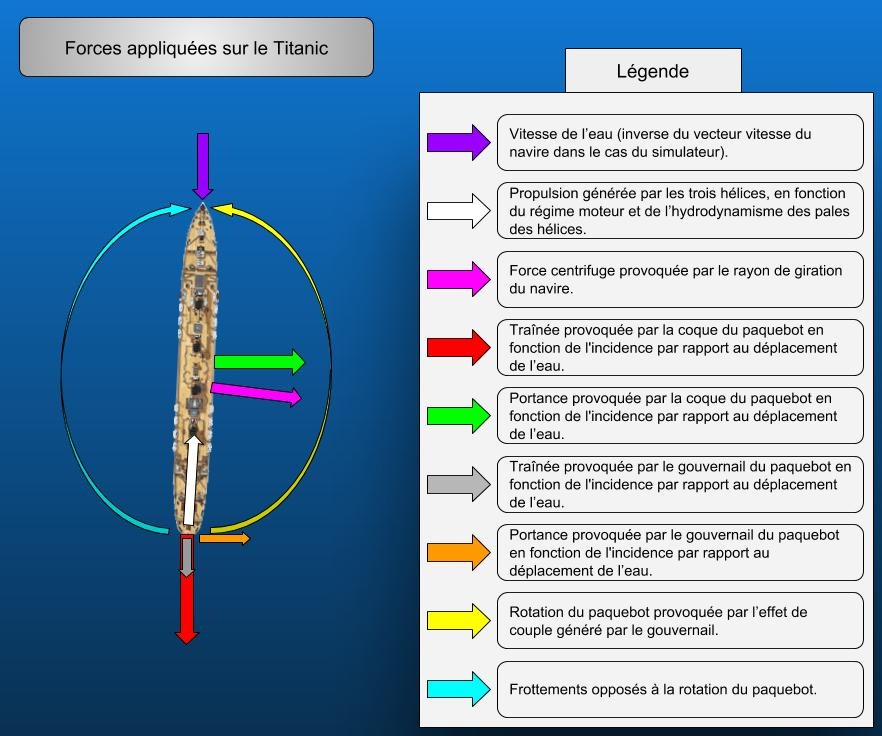
\includegraphics[scale=0.56]{assets/Isaac_vs_Titanic.jpg}
            \label{fig:titanicForces}
        \end{center}
    \end{figure}
    \paragraph{}
    On comprend donc que piloter précisément un navire de cette taille n'est pas simple. Avec toutes les forces physique qui s'appliquent sur lui, il fraudais réaliser beaucoup de calculs pour déterminer les bonnes manœuvres à réaliser. C'est pour cela que nous avons avons choisi d'utiliser la logique floue pour réaliser un pilote automatique, car elle permet d’abstraire tous les phénomènes physique.

    \subsection{Programmation de l'interface}
    Le simulateur naval a été réalisé en langage \textit{C++} en respectant le \textit{design pattern Model View Controller}. L'interface graphique du simulateur a été développé à l'aide du \textit{framework Qt5}.

    \begin{itemize}
        \item La section \textbf{modèle} contient l'ensemble éléments pour réaliser la gestion des phénomènes physique et mécaniques.
        \item La section \textbf{vue} comportent le système de virtualisation (transforment le modèle en scène 2D), ainsi que les composants de l'interface.
        \item La section \textbf{contrôleur} contient tous les actions à réaliser pour chaque composant graphique, ainsi que le pilote automatique.
    \end{itemize}

    \section{Création d'un pilote automatique pour le paquebot}

    \subsection{Objectifs et besoins}

    Le pilote automatique doit permettre au Titanic d’éviter les icebergs en toute sécurité avant même que l'équipage puisse les voir.
    Mais pour éviter les icebergs, il est nécessaire de les détecter. Pour cela nous avons ajouté à la proue trois capteurs lasers indiquant une distance en pourcentage par rapport à sa portée.
    Si un capteur indique 100\% alors il n'y a pas d'objet. En revanche si un capteur indique 50\% alors il y a un objet à la moitié de la potée maximal du capteur. Les trois lasers ont été placé avec un petit angle, afin de pouvoir déterminé le meilleur côté par le quel l'objet peut être évité.

    \begin{figure}[H]
        \begin{center}
            \caption{Schéma présentant les capteurs lasers du Titanic}
            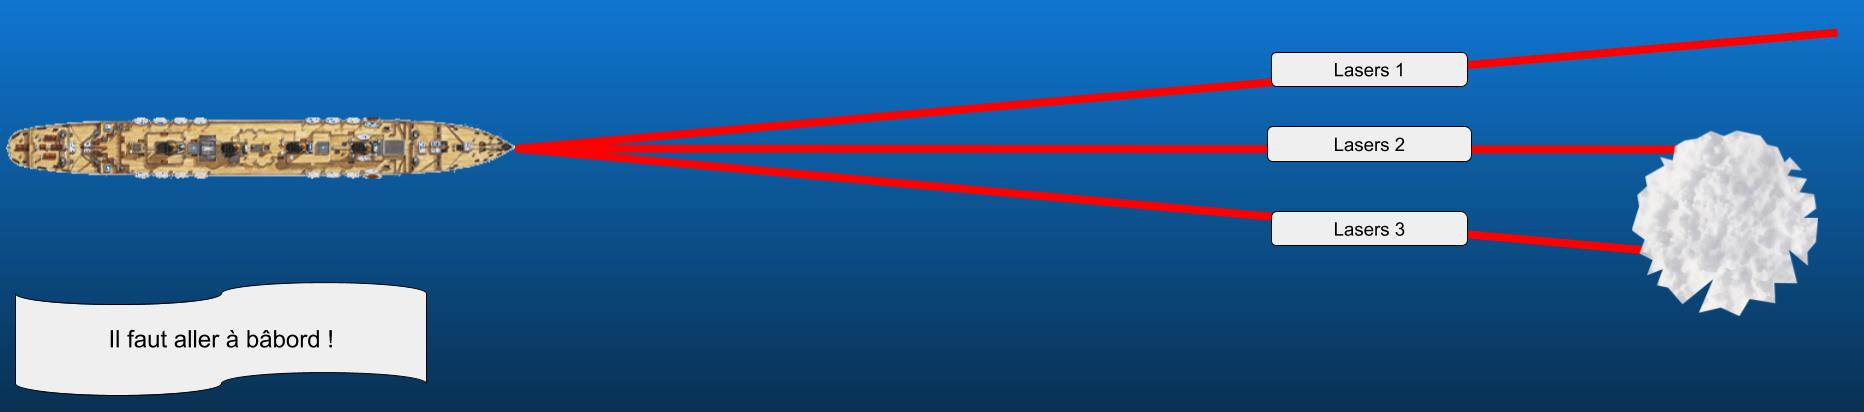
\includegraphics[scale=0.26]{assets/Lasers_Illustration.jpg}
            \label{fig:titanicLasers}
        \end{center}
    \end{figure}

    Pour déterminer la meilleur portée des lasers, il faut connaître la capacité a virer de bord du navire. Dans les meilleurs conditions, le Titanic avait un rayon de giration de 750 m. Nous avons donc réglé la portée des lasers à 800 m, ce qui devrait permettre d’anticiper l’approche des objets suffisamment tôt.

    \subsection{Modélisation du pilote automatique en logique floue}

    Le but : Agir sur l’angle de la barre pour changer (maintenir) le cap pour éviter que le paquebot s’écrase sur l’iceberg.\\
    Le résultat de ce système est un pourcentage. Il correspond à l’angle de la barre pour laquelle le paquebot ne heurtera pas l’iceberg.

    \begin{itemize}
        \item Lorsque la barre aligne le gouvernaille avec l’axe du bateau, elle est a une valeur de 50\%.
        \item Pour une manœuvre à tribord (“droite”), il faut que la barre se situe dans la zone 0\% - 49\%.
        \item Pour une manœuvre à bâbord (“gauche”), il faut que la barre se situe dans la zone 51\% - 100\%.
    \end{itemize}

    \begin{figure}[H]
        \begin{center}
            \caption{Explication de la relation entre la barre et le système flou}
            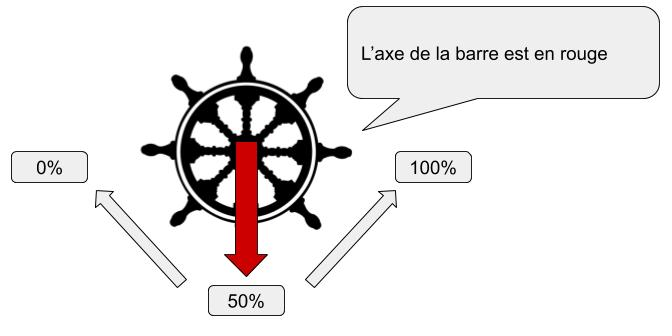
\includegraphics[scale=0.6]{assets/Explications_Barre.jpg}
            \label{fig:helpBar}
        \end{center}
    \end{figure}

    \begin{figure}[H]
        \begin{center}
            \caption{Explication du système floue}
            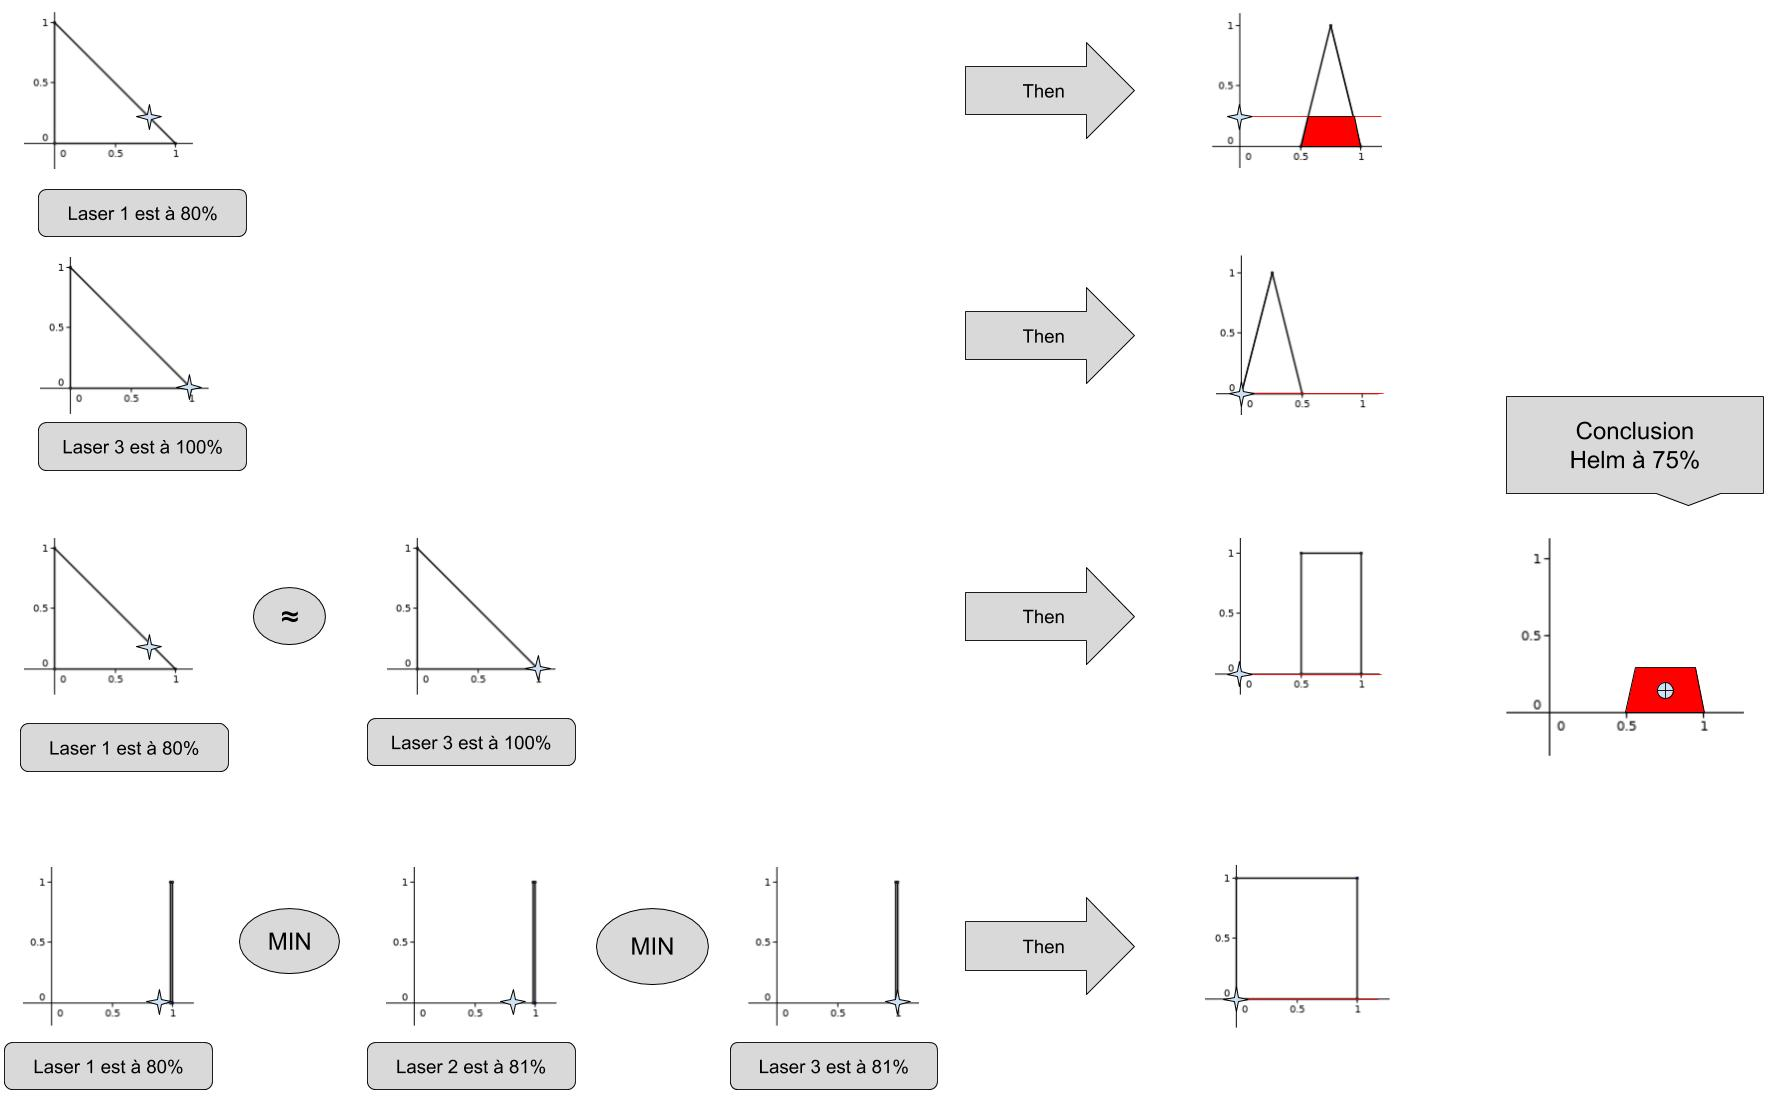
\includegraphics[scale=0.4, angle=90]{assets/Fuzzy_System_Titanic_Helm.jpg}
            \label{fig:systemFuzzy}
        \end{center}
    \end{figure}

    \subsection{Réalisation du système floue à l'aide du \textit{framework}}

    Une fois les conceptes théoriques saisie, nous avons exprimé notre pilote automatique dans le langage de l'interpreteur.

    \begin{figure}[H]
        \begin{center}
            \caption{Code du pilote automatique pour l’interpréteur}
            \lstinputlisting[language=Bash, frame=single]{assets/automatic-pilot.fuzzy}
            \label{fig:codeAutoPilot}
        \end{center}
    \end{figure}


\end{document}
